% !TeX root = ../main.tex

\section{Multirate Processing}
\subsection{Downsampling}
    \begin{LARGE}
        $$
        y(n)=x(nM)
        $$
    \end{LARGE}
    \begin{center}
        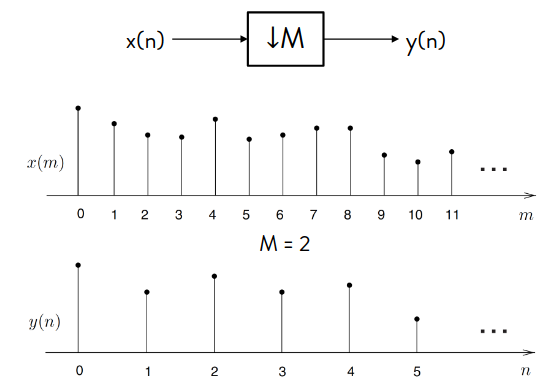
\includegraphics[width=0.9\textwidth]{images/downsampling.png}
    \end{center}
    In the frequency domain, the downsampled is:
    $$
    Y(f)=\frac{1}{M}\sum_{k=0}^{M-1}X\left(\frac{f-k}{M}\right)
    $$
    The DTFT if $y(n)$ is composed of copies of the DTFT of $x(n)$ \textbf{expanded by M and repeated with period 1} in normalized frequency (or $F_s$ in Hertz, or $2\pi$ in angular frequencies)

    \textbf{The gain is reduced by a factor of M}.
    \subsubsection{Aliasing}
    \begin{center}
        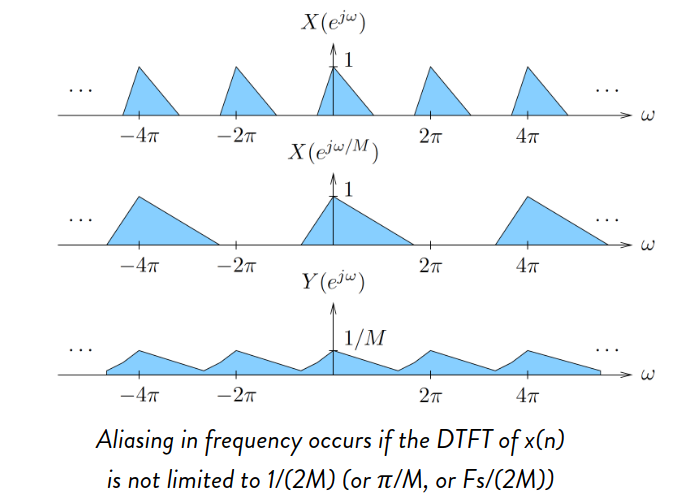
\includegraphics[width=0.9\textwidth]{images/downsampling_aliasing.png}
    \end{center}
    \textbf{Note that in the picture it is not a real signal, not symmetric}.

    There isn't overlap if
    $$
    BM\leq \frac{1}{2}\leftrightarrow B\leq\frac{1}{2M}\leftrightarrow B\leq\frac{\pi}{M}\leftrightarrow B\leq\frac{F_s}{2M}
    $$
    Where $B$ is the first right zero in frequency diagram, the original band of my signal. To avoid aliasing, we introduce a lowpass filter.

    \subsubsection{Decimation}
    Put a lowpass filter, then downsample. We use a lowpass with cutoff of $\frac{1}{2M}$:
    $$
    H(f)=\begin{cases}
        1\qquad |f|\leq\frac{1}{2M}\\
        0\qquad\text{otherwise}
    \end{cases}
    $$
    \begin{center}
        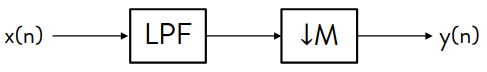
\includegraphics[width=0.5\textwidth]{images/downsampling_lpf.png}
    \end{center}

\subsection{Upsampling}
    Upsampling of a factor L means to insert L -1 zeros between the input signal samples
    \begin{LARGE}
        $$
        y(n)=\begin{Bmatrix}
            x(n/L) & n=kL\\
            0 & \text{otherwise}
        \end{Bmatrix}
        $$    
    \end{LARGE}
    \begin{center}
        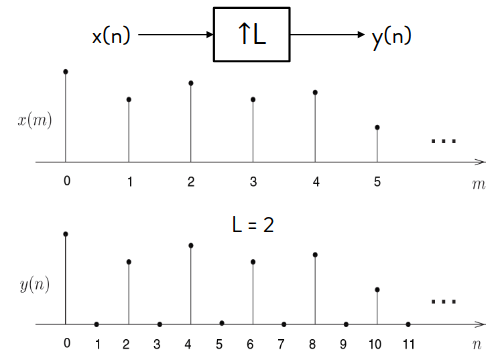
\includegraphics[width=0.9\textwidth]{images/upsampling.png}
    \end{center}
    In the frequency domain:
    $$
    Y(f)=X(fL)
    $$
    Upsampling compresses the DTFT by a factor of $L$, \textbf{if we upsampled a sinusoid, its DFT will repeat the pulses every $L$, same goes for the symmetric pulses}.


    \subsubsection{Replicas}
    \begin{center}
        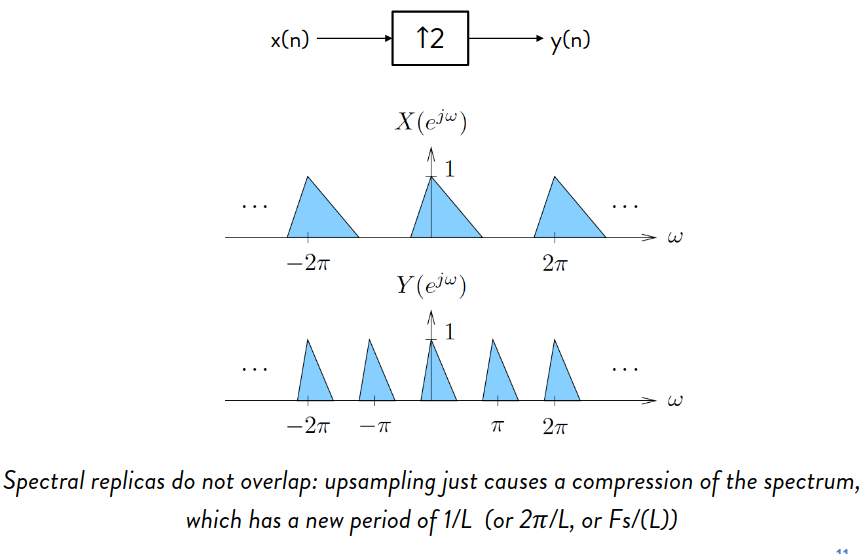
\includegraphics[width=0.9\textwidth]{images/upsampling_replica.png}
    \end{center}

    \subsubsection{Interpolation}
    Put a lowpass filter \textbf{after} upsampling. We use a lowpass with cutoff of $\frac{1}{2L}$, in this way we remove replicas:
    $$
    H(f)=\begin{cases}
        L\qquad|f|\leq\frac{1}{2L}\\
        0\qquad\text{otherwise}
    \end{cases}
    $$
    \begin{center}
        \includegraphics[width=0.5\textwidth]{images/upsampling_Interpolation.png}
    \end{center}
    \textbf{After lpf, MULTIPLY AGAIN THE SIGNAL BY L}

\subsection{Rational sampling rate conversion: noninteger factor}
    Cascade interpolator wih a decimator
    \begin{center}
        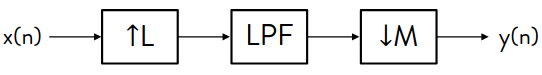
\includegraphics[width=0.5\textwidth]{images/rationalsampling.png}
    \end{center}
    The lowpass dilter is:
    $$
    H(f)=\begin{cases}
        L\qquad|f|\leq\min\Brackets{\frac{1}{2L},\frac{1}{2M}}\\
        0\qquad\text{otherwise}
    \end{cases}
    $$
